\section{Channel Parameters}
\lecture{18 Mar.}

Let us define a few channel parameters that will aid our analysis of channels latter on.

We especially consider those that respect the structure of the decomposition of a compound channel into BSCs. Consider an arbitrary BMSC $W=\sum_{i}a_i\mathrm{BSC}(p_i)$, let us define
\begin{definition}[Channel Parameters]
    \begin{itemize}
        \item \textbf{Conditional Entropy}:
        \begin{align}
            &H(W) \defeq \sum_{i}a_i H\left(\mathrm{BSC}(p_i)\right),\\
            &H\left(\mathrm{BSC}(p)\right) \defeq h_b(p) = -p\lg p - \bar{p}\lg\bar{p}.
        \end{align}
        The function $h_b$ is the binary entropy, and $\bar{p}=1-p$. Note that the capacity of a BSC is $C(\mathrm{BSC}(p)) \defeq 1-H(\mathrm{BSC}(p))$.
        \item \textbf{Bhattacharyya Parameter}:
        \begin{align}
            &Z(W) \defeq \sum_{i}a_i Z\left(\mathrm{BSC}(p_i)\right),\\
            &Z\left(\mathrm{BSC}(p)\right) \defeq 2\sqrt{p\bar{p}}.
        \end{align}
        Note that when $p\rightarrow0$ or $1$, $Z\rightarrow0$; when $p\rightarrow\frac{1}{2}$, $Z\rightarrow1$.
        \item \textbf{Total Variation Distance}:
        \begin{align}
            &T(W) \defeq \sum_{i}a_i T\left(\mathrm{BSC}(p_i)\right),\\
            &T\left(\mathrm{BSC}(p)\right) \defeq \abs{1-2p} = \abs{\frac{1}{2}-p} + \abs{\frac{1}{2}-\bar{p}} = \abs{p-\bar{p}}.
        \end{align}
        This parameter is also a symmetric one. Furthermore, it measures how far away our distribution is from the uniform distribution.
        \item \textbf{Bit Error Probability}:
        \begin{align}
            &P_e(W) \defeq \sum_{i}a_i P_e\left(\mathrm{BSC}(p_i)\right),\\
            &P_e\left(\mathrm{BSC}(p)\right) \defeq 2\min\{p,\bar{p}\}.
        \end{align}
        Where does the mysterious 2 come from? Observe the following example for an explanation.
    \end{itemize}
\end{definition}

\begin{example}
    Consider a channel $\mathrm{BEC}(x) = \bar{x}~\mathrm{BSC}(0) + x~\mathrm{BSC}(1/2)$. The error probability actually depends on how we want to decode it. If one simply gives up when seeing an erasure output, the error probability will be $P_e(\mathrm{BSC}(x))=x$. However, if we try really hard and simply guess when receiving an erasure, the error probability will be, under a uniform prior, $P_e(\mathrm{BSC}(x))=x/2$.

    It is of a notational agreement that when considering the channel parameter $P_e$, we let it be characterizing the error probability when we simply give up. Henceforth, we have
    \begin{equation*}
        P_e\left(\mathrm{BEC}(x)\right) = \bar{x}~P_e\left(\mathrm{BSC}(0)\right) + x~P_e\left(\mathrm{BSC}(1/2)\right) = \bar{x}\cdot0 + x\cdot2\cdot\frac{1}{2} = x.
    \end{equation*}
    The benefit of this notational agreement will be the fact that $P_e\left(\mathrm{BSC}(p)\right)\in[0,1]$ for all $p$, and so is their convex combination. This is the same for all other parameters we just introduced, they all lie in the interval $[0,1]$.
\end{example}
These parameters will be shown to be really useful in characterizing how good a channel is. And by converting between different parameters, many of the properties of a channel can be characterized as well.

\begin{figure}[H]
    \centering
    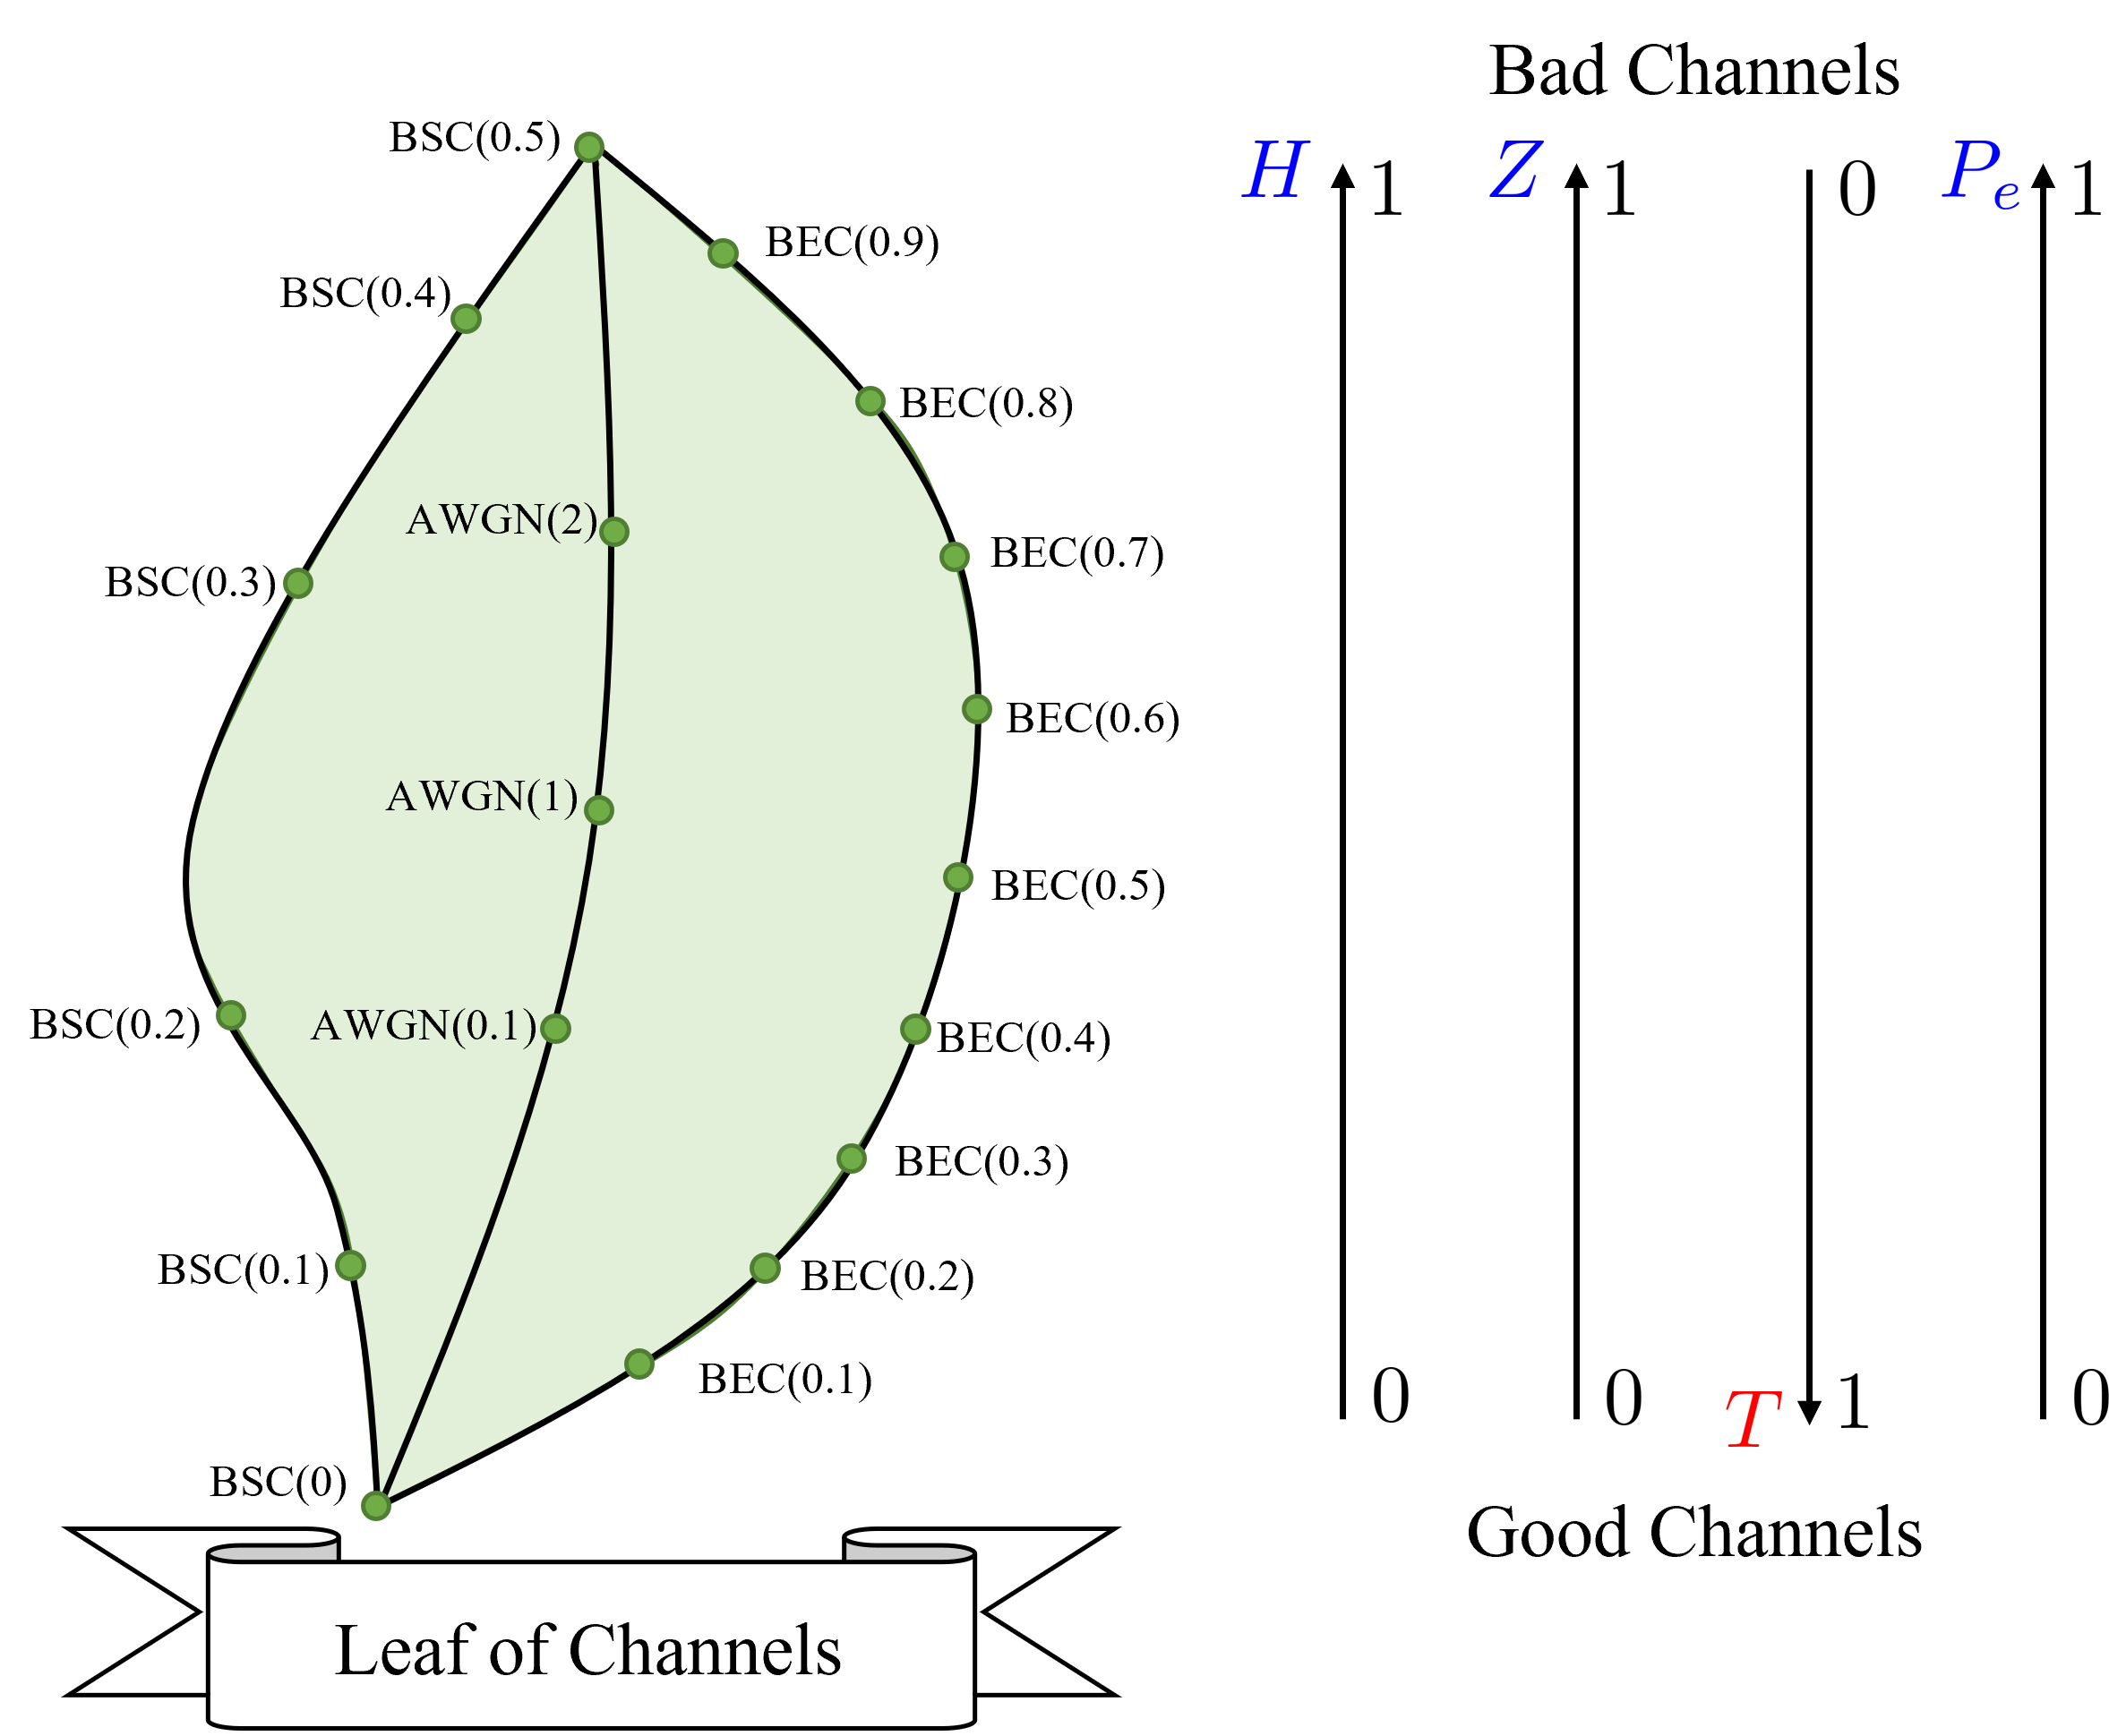
\includegraphics[width=0.8\linewidth]{figures/w5_leaf_of_channels.png}
    \caption{Leaf of channels representing the trend of channels from bad to good. The measures of the trend of how good a channel is are the channel parameters, coinciding on the value of 0 and 1 on $\mathrm{BSC}(0)$ and $\mathrm{BSC}(0.5)$ for the parameters $H$, $Z$, $P_e$ (measuring how bad a channel is), and vice versa for $T$.}
\end{figure}


\subsection{Inequalities of Channel Parameters}
For a more exhaustive list of results and proofs of the topic in this subsection, please refer to the papers ``A note on some inequalities used in channel polarization and polar coding'' \cite{Inequalities_Channel_Polarization} and ``Binary Polar Codes Based on Bit Error Probability'' \cite{Binary_PC_Bit_Err_Prob}.

\begin{theorem}
    For all BMSC $W$, we have
    \begin{equation}
        Z(W)^2\le H(W) \le Z(W).
    \end{equation}
\end{theorem}
\begin{proof}
    By plotting the respective values for the simple case $W=\mathrm{BSC}(p)$, we can see the above inequality holds true. Furthermore, the two inequalities still holds true under convex combination, but the first needs to further utilize the fact that $y=x^2$ is a convex functions.
\end{proof}
\begin{theorem}
    For a BMSC $W$,
    \begin{equation}
        1-T(W) \le H(W) \le h_b\left(\frac{1-T(W)}{2}\right)
    \end{equation}
\end{theorem}
\begin{proof}
    The proof is similar to the previous one, where one first show the inequality holds for BSCs, which is trivial. Then the first inequality is easily extended under convex combination. The second inequality still holds true since $h_b(p)$ is concave.
\end{proof}

\begin{remark}
    BEC is really special in that its $H=Z=P_e=1-T$ for all possible erasure probabilities.

    This is easy to show since that BECs are convex combination of the extremal BSCs, i.e., $\mathrm{BSC}(0)$ and $\mathrm{BSC}(1/2)$. The channel parameters coincide on these extremals.
\end{remark}

With the two inequalities above, we can actually bound regions of possible $(H,Z)$ and $(H,T)$ pairs as shown in \autoref{fig:w5_channel_parameter_region} below. Note that the upper curve in the $H$-$Z$ plot is not $Z^2=X$, it is not optimal.

\begin{figure}[H]
   \centering
   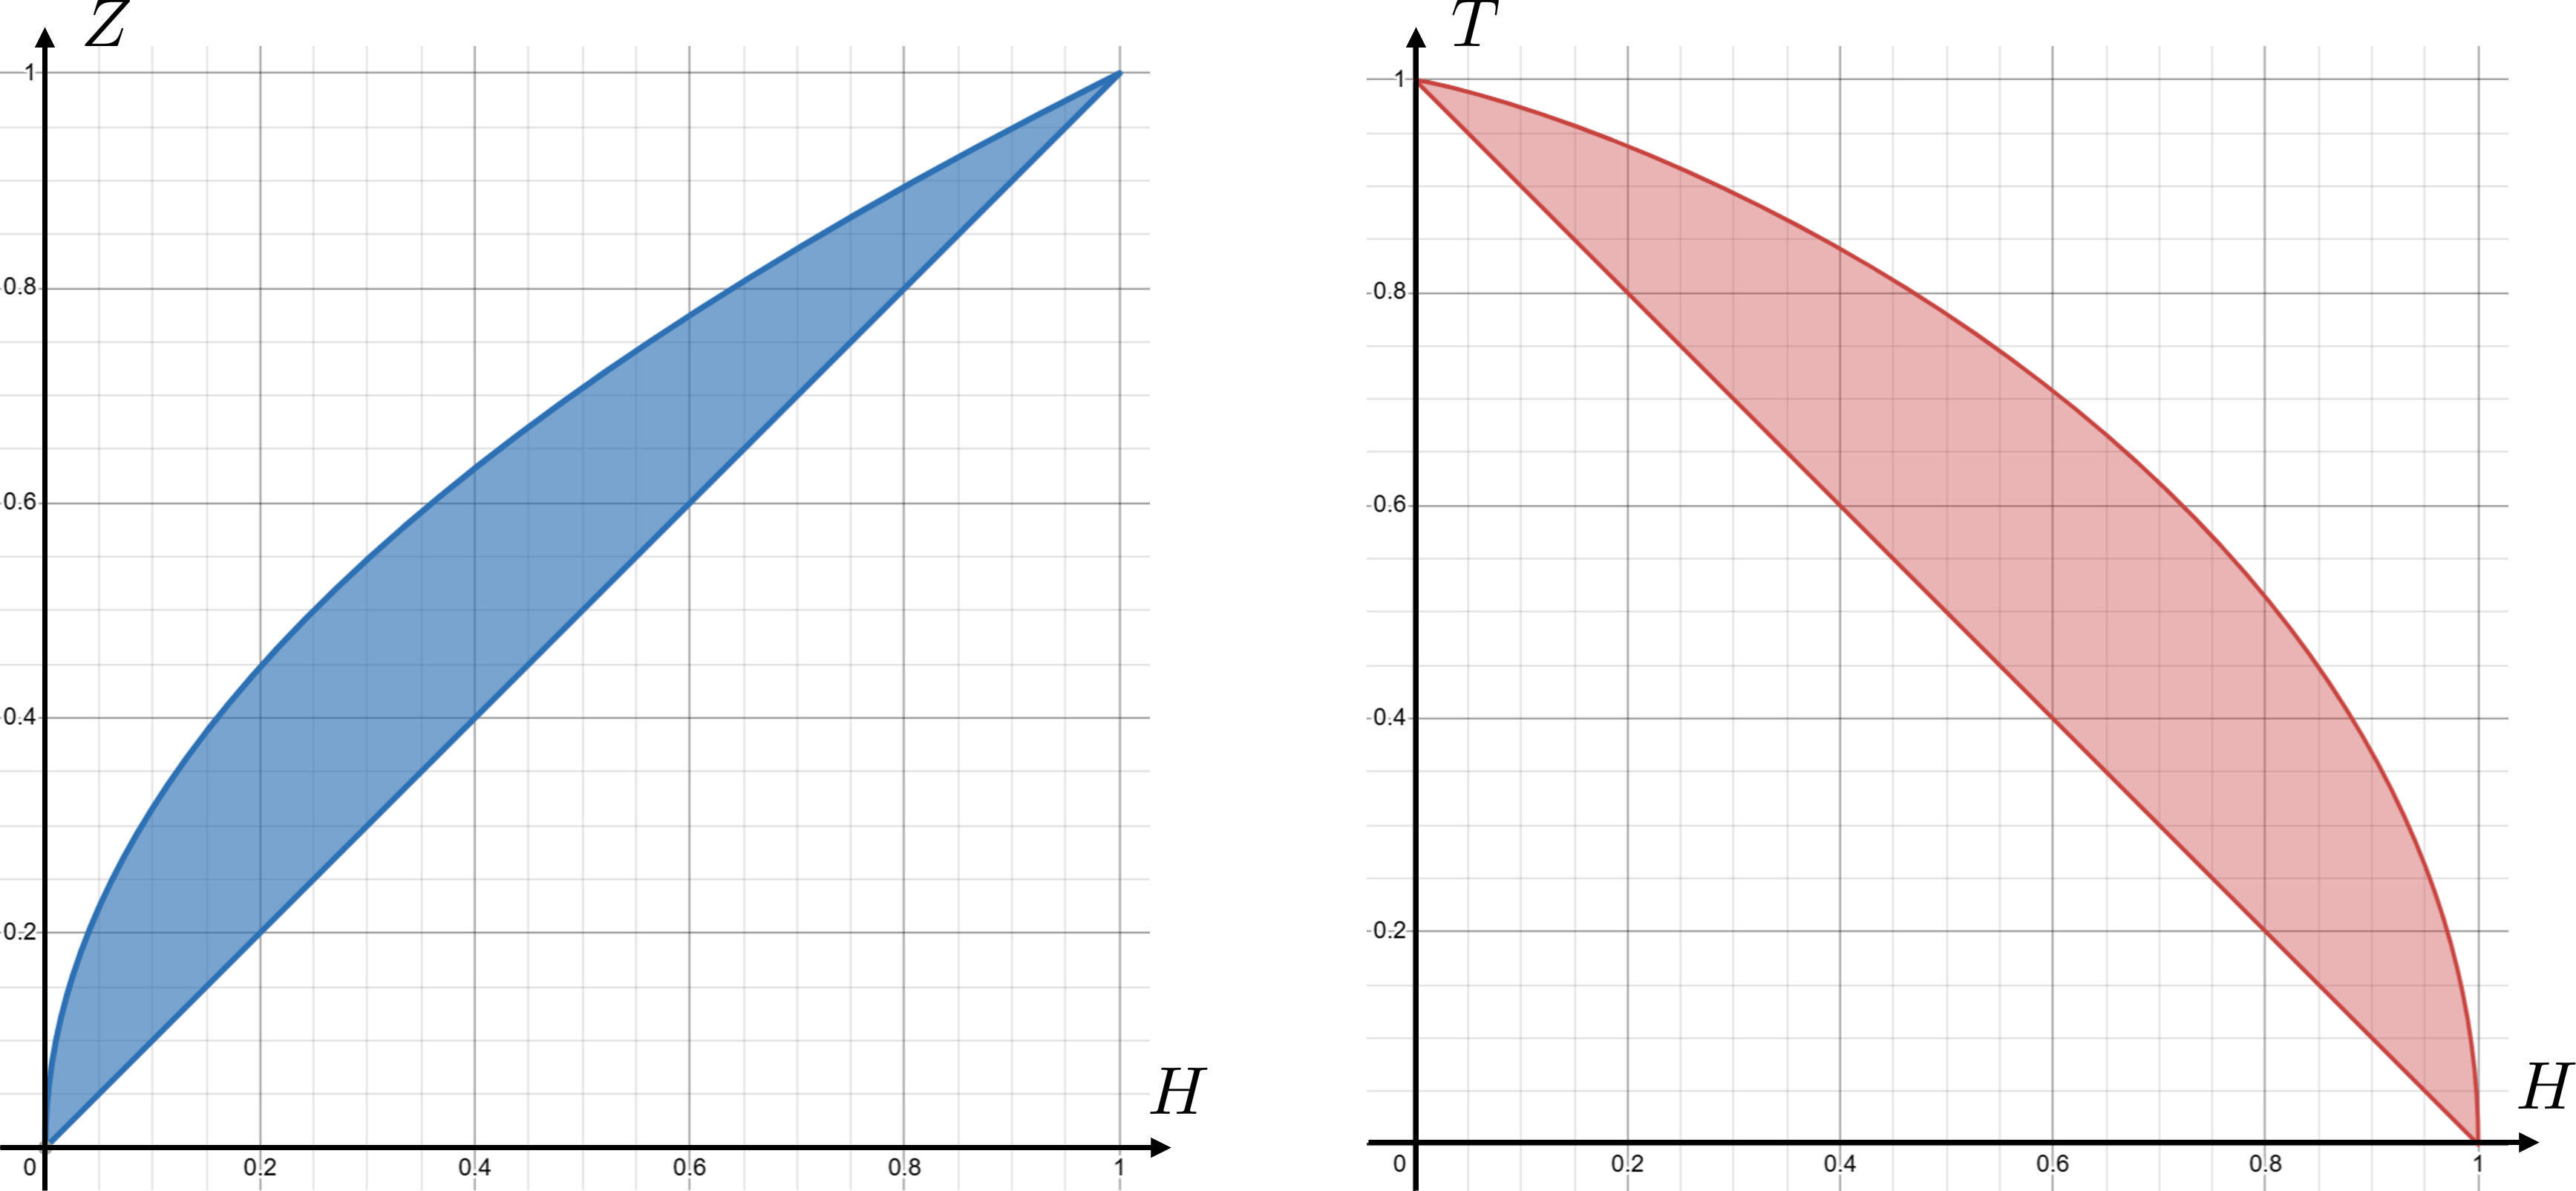
\includegraphics[width=0.8\linewidth]{figures/w5_region_parameter.png}
   \caption{Possible combinations of channel parameters.}
   \label{fig:w5_channel_parameter_region}
\end{figure}


\subsection{Channel Parameters as Martingales} 
Why do we study all these parameters? Because each one of them is good at one or two aspects, and only when combined together do we learn the full picture.
\begin{theorem}[Channel Parameters of Polarized Sub-Channels] \label{thm:channel_param_martingale}
    The following relations hold for the polarized sub-channels $W^+$ and $W^-$ of the BMSC $W$:
    \begin{align}
        &H(W^+) + H(W^-) = 2H(W),\\
        &Z(W^+) = Z(W)^2,\\
        &Z(W^-) \le 2Z(W) - Z(W)^2,\\
        &T(W^-) = T(W)^2,\\
        &T(W^+) \le 2T(W) - T(W)^2.
    \end{align}
    Hence, we know that for $s_{1:k}\in\{+,-\}^k$ $H(W^{s_{1:k}})$ is a martingale, and both $Z(W^{s_{1:k}})$ and $T(W^{s_{1:k}})$ are supermartingales. Furthermore, we have the more general results of
    \begin{align}
        Z(W_1\ostar W_2) &= Z(W_1)\cdot Z(W_2), \\
        T(W_1\boxstar W_2) &= T(W_1)\cdot T(W_2)
    \end{align}
    for channels $W_1$ and $W_2$.
\end{theorem}

\begin{remark}[Helliger Affinity]
    The Helliger affinity of a channel $W$ is defined as
    \begin{equation}
        Z_\alpha(W) = 2p^\alpha \bar{p}^{1-\alpha}.
    \end{equation}
    It is a (R\'enyi-like) generalization to the Bhatacharyya parameter (at $\alpha=1/2)$, also satisfying the multiplicative property of
    \begin{equation}
        Z_\alpha(W_1\ostar W_2) = Z_\alpha(W_1)\cdot Z_\alpha(W_2).
    \end{equation}
\end{remark}

The proof to parts of Theorem \autoref{thm:channel_param_martingale} will be shown later. But for now, let us analyze the consequences the martingales generated by the polarization process brought.
\begin{theorem}[Martingale Convergence Theorem]
    If $\{M_t\}$ is a bounded\footnote{For supermartingales $M_t$, the boundedness is in the sense of that $\sup_t \mathbb{E}[-\min(M_t,0)]<\infty$.} supermartingale / submartingale, then its limit exists: $M_t\xrightarrow{\text{a.s / $L^1$}}M_\infty$.
\end{theorem}
\begin{theorem}[Optional Stopping Time]
    For supermartingale $\{M_t\}$, we have $\mathbb{E}[M_\sigma] \le M_0$.

    For submartingale $\{M_t\}$, we have $\mathbb{E}[M_\sigma] \ge M_0$.
\end{theorem}
\begin{theorem}[Doob's Maximum Inequality]
    If $M_t\ge 0$ is a supermartingale, then $\mathrm{Pr}\{\max_tM_t\ge B\} \le M_0/B$.

    If $M_t\le 0$ is a submartingale, then $\mathrm{Pr}\{\max_tM_t\le -B\} \le -M_0/B$.
\end{theorem}

When applied to the channel parameters, one can have the following analyses:
\begin{example}
    Take the Bhattacharyya parameter as an example, define the Bhattacharyya martingale as
    \begin{equation}
        Z_0\defeq Z(W),\;Z_k\defeq Z(W^{s_{1:k}})\;\;\;\;\;(s^k\in\{+,-\}^k \text{ uniformly and random}).
    \end{equation}
    By the martingale convergence theorem, a limit should exist. It can be shown that $Z_\infty\in\{0,1\}$. Then we have
    \begin{equation*}
        \mathrm{Pr}\{Z_\infty=1\} = H_0 = H(W) \le Z_0.
    \end{equation*}
    Weirdly enough, one would expect the left hand side be equal to $Z_0$ by mirroring the proof from martingale. However, since now $Z_k$ is a supermartingale, the analysis should be: since $Z(W)\approx1$ if and only if $H(W)\approx 1$, we have
    \begin{equation}
        \mathrm{Pr}\{Z_\infty=1\} = \mathrm{Pr}\{H_\infty=1\} = H_0.
    \end{equation}
\end{example}

In fact, we have
\begin{equation}
    H_\infty = Z_\infty = 1 - T_\infty = P_{e,\infty}.
\end{equation}
Similarly, we have that as $k\rightarrow\infty$, $T_k$ converges to $T_\infty\in\{0,1\}$, with $\mathrm{Pr}\{T_\infty=1\} = 1-H_0$.

\subsection{Polar Decoder under Parallel and Serial Combination} \label{sec:w5_polar_dec_par_ser}
The general decoding scheme for a polar decoder is abstractly illustrated as below:
\begin{figure}[H]
    \centering
    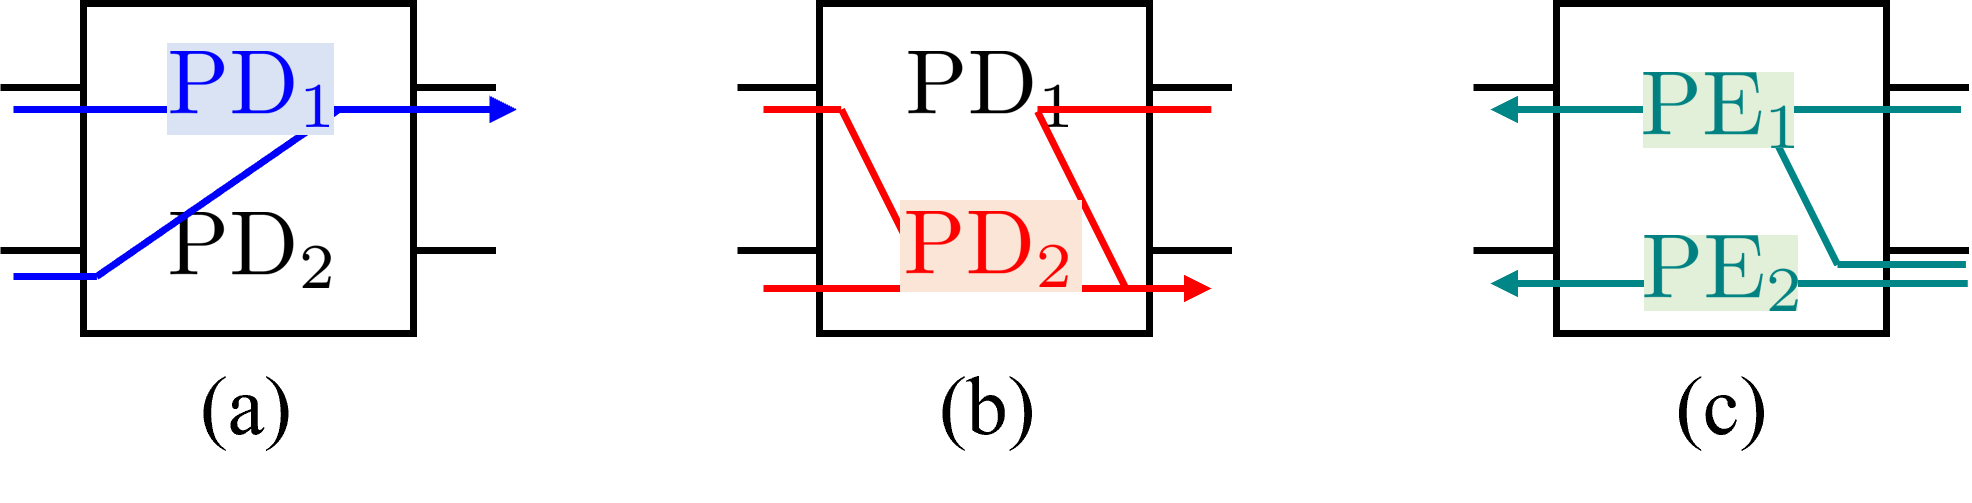
\includegraphics[width=0.6\linewidth]{figures/w5_dec_scheme.png}
    \caption{The three steps for decoding of polar code.}
\end{figure}
The decoding steps are implemented in real life by analyzing the likelihood ratio. To derive the likelihood ratio of the input symbols, let us introduce a new notion.
\begin{definition}[Posterior Probability Representation of Uncertain Symbols]
    If one were to guess the input $x\in\mathcal{X}=\{0,1\}$ given the received $y\in\mathcal{Y}$, the only crucial information are the posterior probabilities. Hence, one should represent $y$ by the pair of posterior probabilities
    \begin{equation}
        \left(W(0\vert y), W(1\vert y)\right)
    \end{equation}
    with a uniform prior, where the channel is $W:\mathcal{X}\rightarrow\mathcal{Y}$ .
\end{definition}

\begin{example}
    Consider the channel below:
    \begin{figure}[H]
        \centering
        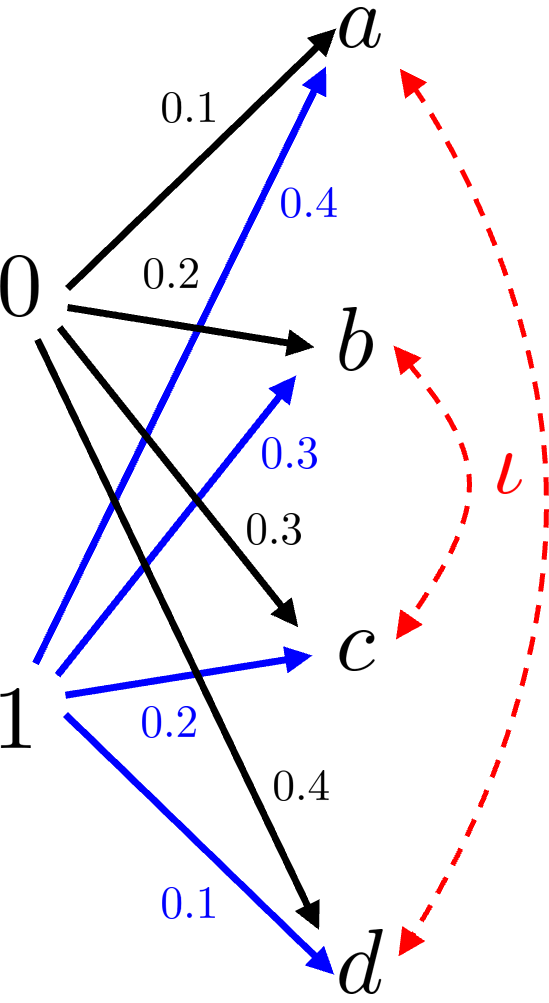
\includegraphics[width=0.2\linewidth]{figures/w5_post_rep1.png}
        \caption{Example of a BMSC for posterior representation.}
    \end{figure}
    In stead of ``$a$'', use the representation
    \begin{equation*}
        \left(W(0\vert a,W(1\vert a)\right) = \left(\frac{0.1}{0.1+0.4},\frac{0.4}{0.1+0.4}\right) = \left(\frac{1}{5},\frac{4}{5}\right).
    \end{equation*}
    Similarly, instead of ``$b$'', use $(2/5,3/5)$; instead of ``$c$'', use $(3/5,2/5)$; instead of ``$d$'', use $(4/5,1/5)$.
\end{example}
\begin{example}
    Consider the channel below
    \begin{figure}[H]
        \centering
        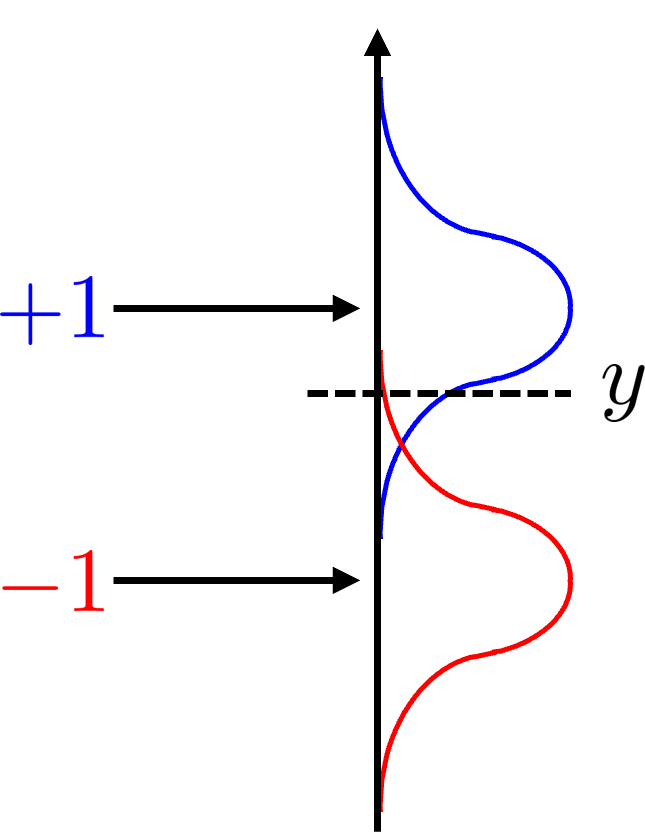
\includegraphics[width=0.2\linewidth]{figures/w5_post_rep2.png}
        \caption{Example of posterior representation on continuous random variables.}
    \end{figure}
    Since probabilities of outputs no longer make sense, we utilize the probability densities instead. Let the $\varphi(y)$ be the probability density function of the standard normal distribution. Then since $W(y\vert1)=\varphi(y-1)$ and $W(y\vert-1)=\varphi(y+1)$, we have the posterior representation of the output $y$ being
    \begin{equation*}
        \left(W(1\vert y),W(-1\vert y)\right) = \left(\frac{\varphi(y-1)}{\varphi(y-1)+\varphi(y+1)},\frac{\varphi(y+1)}{\varphi(y-1)+\varphi(y+1)}\right).
    \end{equation*}
\end{example}
Now let utilize both the posterior representation and the channel parameters introduced in the analysis of parallel and serial combination of channels.

\paragraph{Posterior Representation \& Parallel Combination:}

If one sends $X=x$ through $W$ and $W'$, and obtained posterior representations $(\alpha,\bar{\alpha})$ and $(\beta,\bar{\beta})$, respectively. Then what is the posterior probability of $x$ now? This can be readily solved by pretending $W$ and $W'$ as BSCs, and consider the figure below:
\begin{figure}[H]
    \centering
    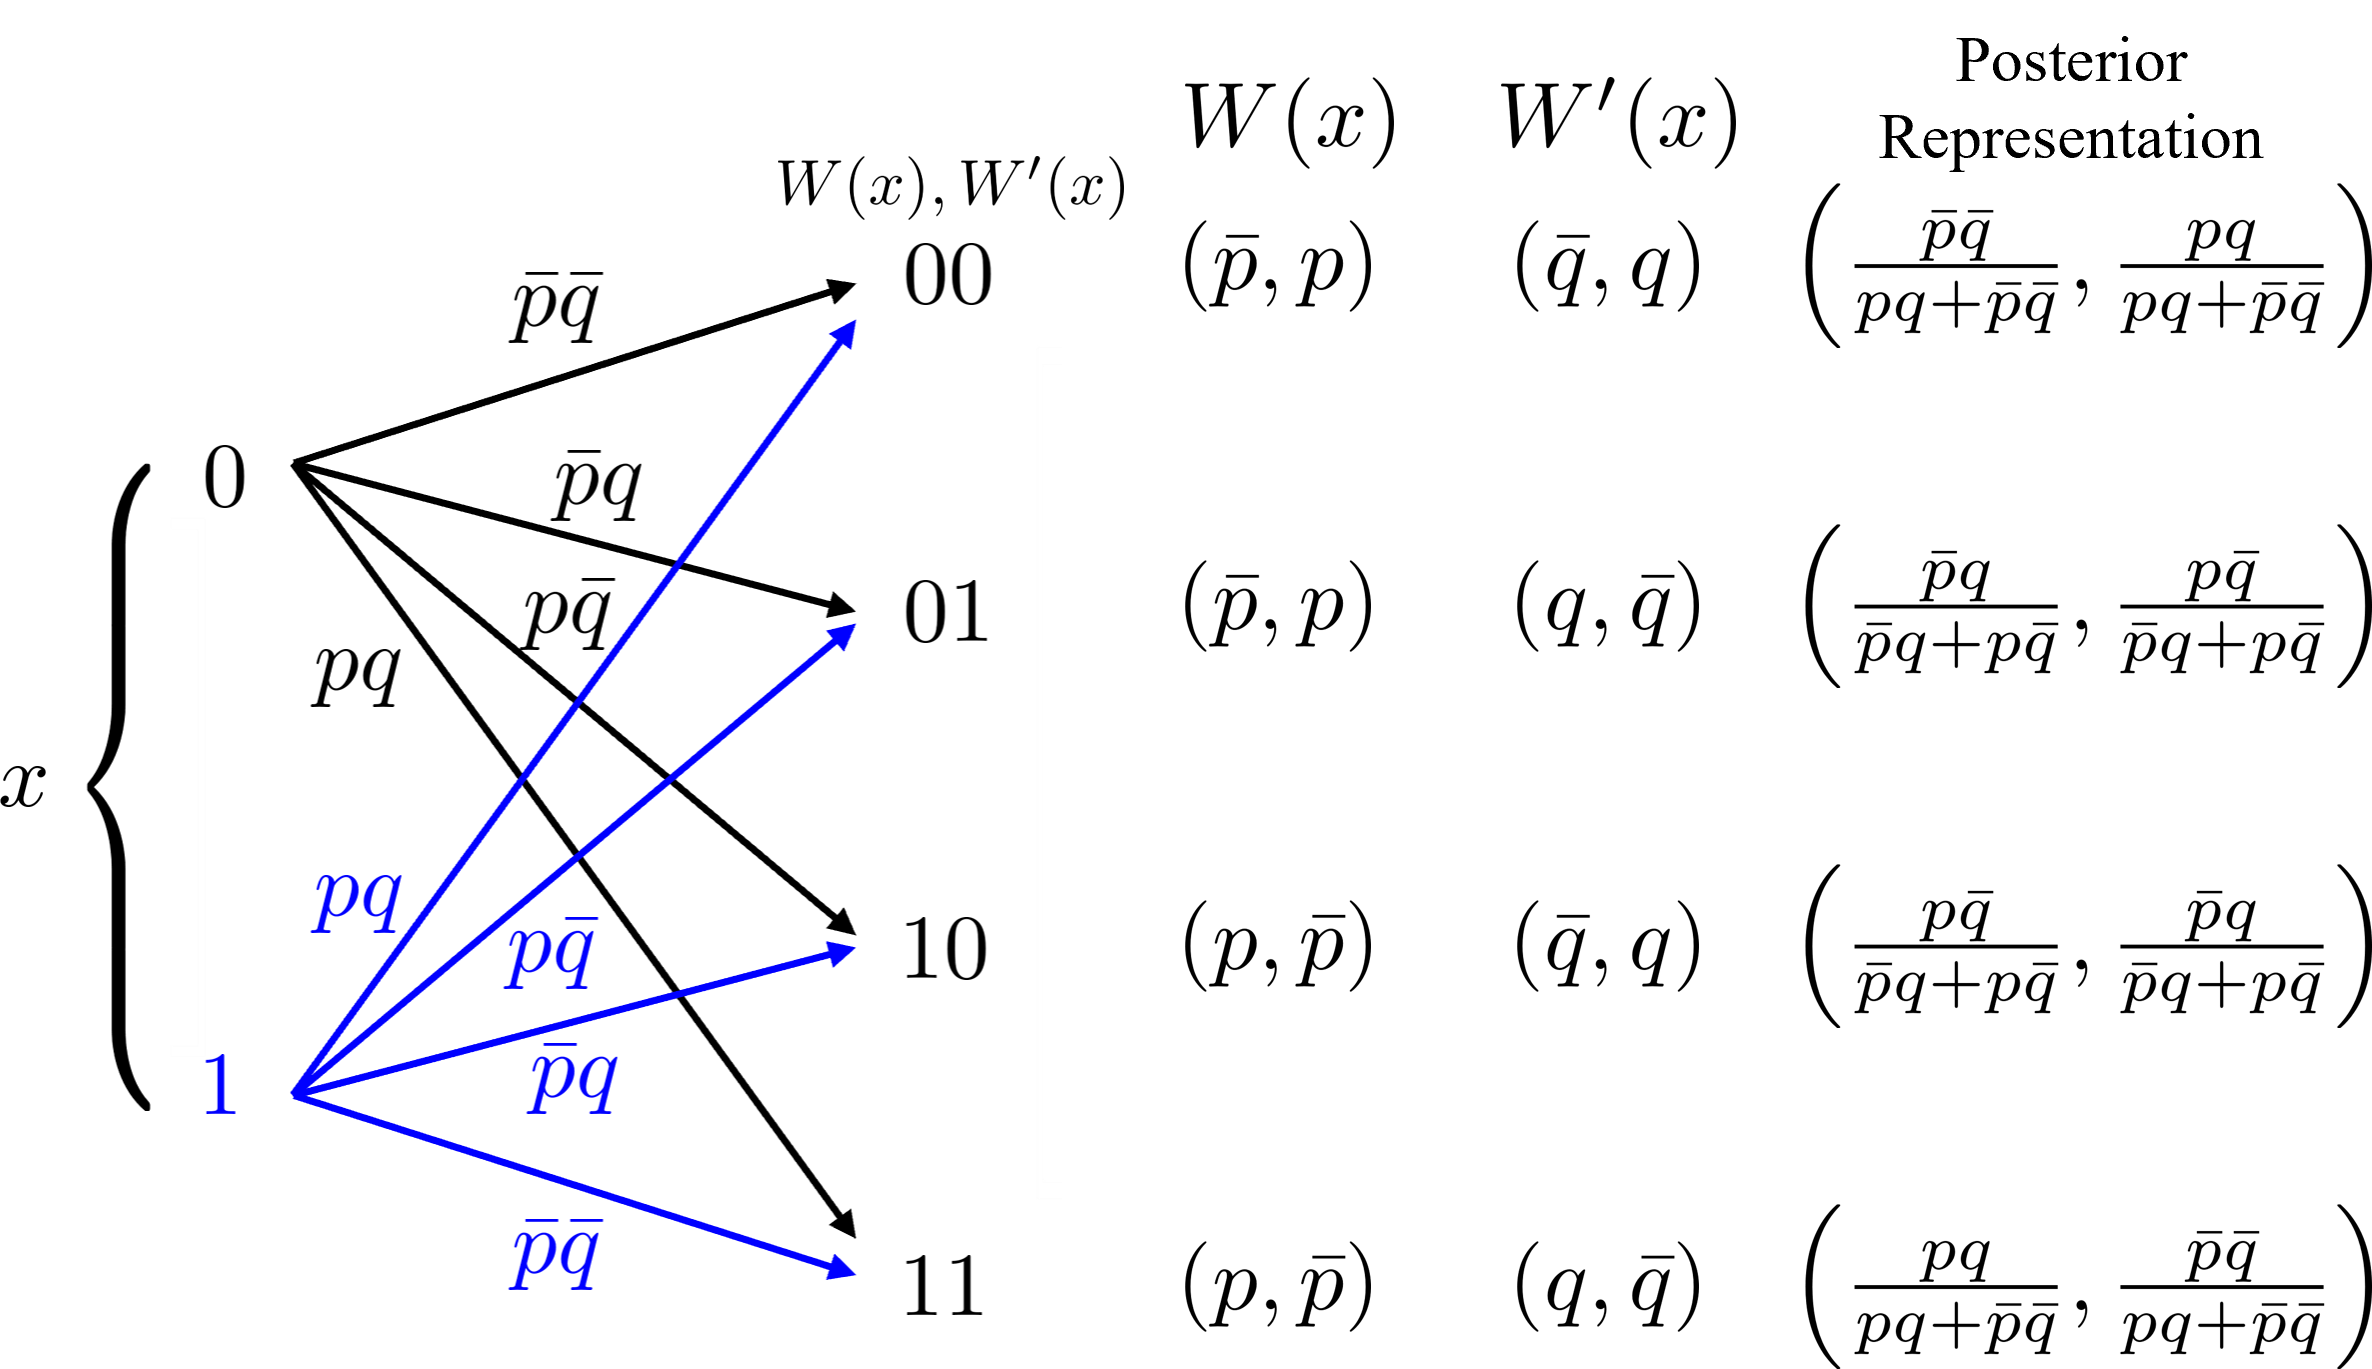
\includegraphics[width=0.7\linewidth]{figures/w5_post_parallel.png}
    \caption{Posterior representation for parallel combination of BSC's.}
\end{figure}
It is easily seen that if the received symbols are $(\alpha,\bar{\alpha})$ and $(\beta,\bar{\beta})$, they amount to a posterior representation of
\begin{equation}
    (\gamma,\bar{\gamma}) \defeq \left(W(x=0\vert W(x),W'(x)), W(x=1\vert W(x),W'(x))\right) = \left(\frac{\alpha\beta}{\alpha\beta + \bar{\alpha}\bar{\beta}} , \frac{\bar{\alpha}\bar{\beta}}{\alpha\beta + \bar{\alpha}\bar{\beta}}\right).
\end{equation}
Consider the likelihood ratios, especially, we can easily see that they are multiplicative!
\begin{equation}
    \frac{\gamma}{\bar{\gamma}} = \frac{\alpha}{\bar{\alpha}} \cdot \frac{\beta}{\bar{\beta}}.
\end{equation}
This serves as a mnemonic for one to remember the channel combination rule.

We hence have the following result:
\begin{theorem}[Bhattacharyya Parameter under Parallel Combination]
    For channels $W_1$ and $W_2$, we have
    \begin{equation}
        Z(W_1\ostar W_2) = Z(W_1)\cdot Z(W_2).
    \end{equation}
    Especially when $W_1=W_2=W$, we have
    \begin{equation}
        Z(W^+) = Z(W)^2.
    \end{equation}
\end{theorem}
\begin{proof}
    Since any BMSC can be decomposed into a convex combination of BSCs, we only need to proof the theorem above for parallel combination of BSCs. This can be directly proven by plugging in \autoref{w3:BSC_parallel}. 
    
    However, also observe that for a general channel $W=\sum_i a_i \mathrm{BSC}(p_i)$. By treating the output symbols $y_i$ in their posterior representations $(\alpha(y_i),\bar{\alpha}(y_i)) = (p_i,\bar{p}_i)$ as a random variable with distribution derived from sending only 1 as the input, we can construct the following expectation:
    \begin{equation*}
        Z(W) = \sum_i a_i\cdot2\sqrt{p_i\bar{p}_i} = \sum_i a_i\left(p_i\sqrt{\bar{p}_i/p_i} + \bar{p}_i \sqrt{p_i/\bar{p}_i}\right) = \mathbb{E}\left[\sqrt{\bar{\alpha}/\alpha}\right].
    \end{equation*}
    Then the result above can be simply derived from
    \begin{equation*}
        Z(W_1\ostar W_2) = \mathbb{E}\left[\sqrt{\gamma/\bar{\gamma}}\right] = \mathbb{E}\left[\sqrt{\alpha/\bar{\alpha}}\right] \cdot \mathbb{E}\left[\sqrt{\beta/\bar{\beta}}\right] = Z(W_1) \cdot Z(W_2).
    \end{equation*}
\end{proof}


\paragraph{Posterior Representation \& Serial Combination:}

If one sent $x$ through $W$ obtaining $(\alpha,\bar{\alpha})$ and sent $y$ through $W'$ obtaining $(\beta,\bar{\beta})$. Then what is the posterior representation to $x+y$? Similarly, pretend $W$ and $W'$ to be BSCs and consider the figure below:
\begin{figure}[H]
    \centering
    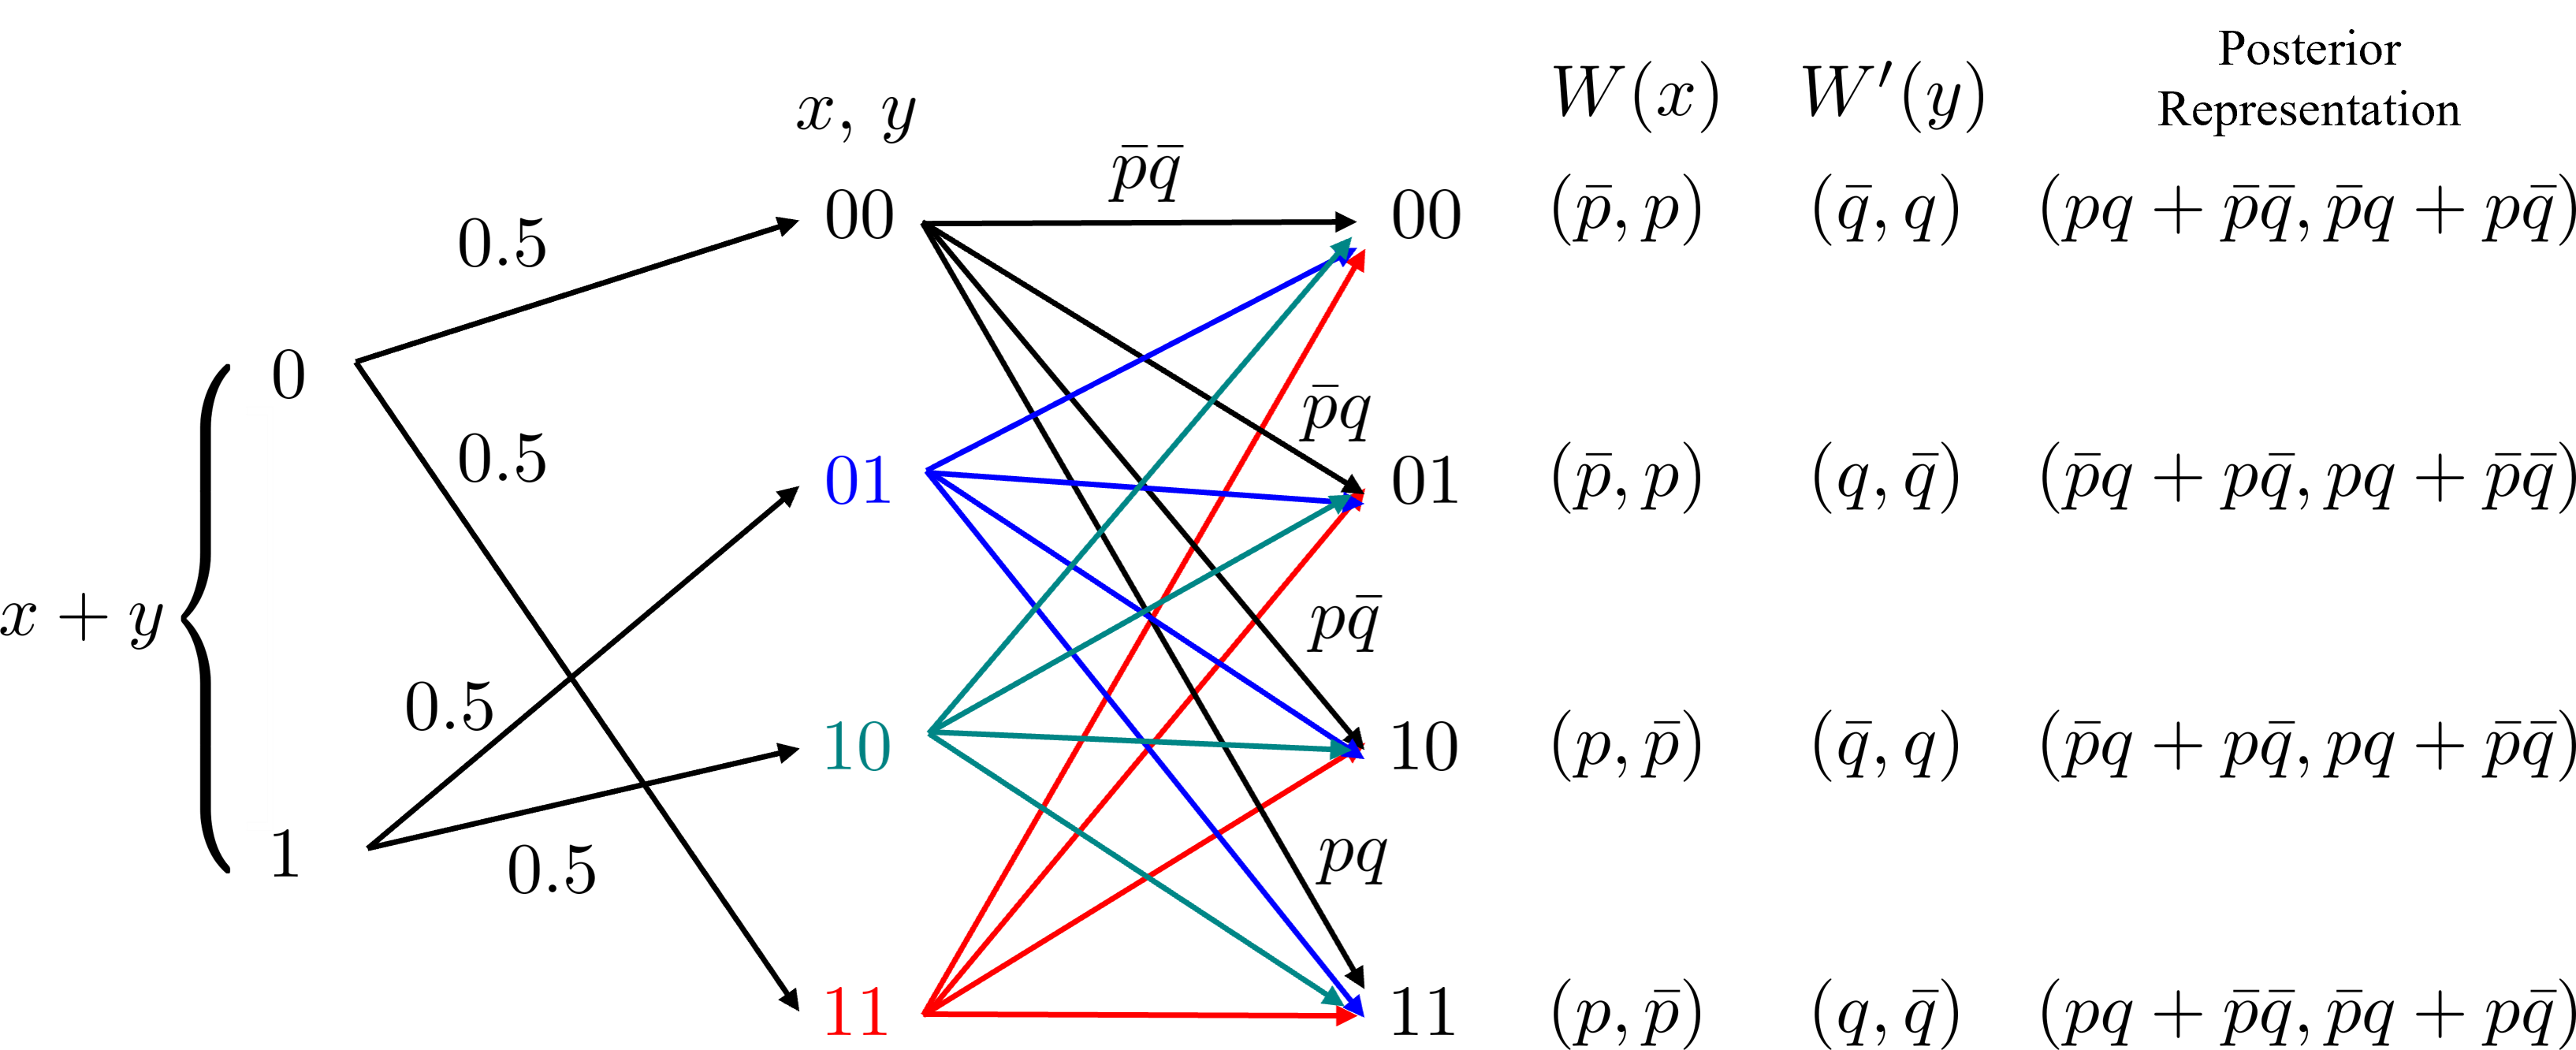
\includegraphics[width=0.9\linewidth]{figures/w5_post_serial.png}
    \caption{Posterior representation for serial combination of BSC's.}
\end{figure}
One can see that if the received symbols are $(\alpha,\bar{\alpha})$ and $(\beta,\bar{\beta})$, they amount to a posterior representation of
\begin{equation}
    (\gamma,\bar{\gamma}) \defeq \left(W(x+y=0\vert W(x),W'(y)), W(x+y=1\vert W(x),W'(y))\right) = \left(\alpha\beta + \bar{\alpha}\bar{\beta},\bar{\alpha}\beta + \alpha\bar{\beta}\right).
\end{equation}
One can also observe that the signed variation distance is multiplied:
\begin{equation}
    (\gamma-\bar{\gamma}) = (\alpha-\bar{\alpha}) \cdot (\beta-\bar{\beta}).
\end{equation}
This serves as yet another mnemonic.

The following result follows suit:
\begin{theorem}{Total Variation Distance under Serial Combination} \label{thm:w5_TV_multiply}
    For channels $W_1$ and $W_2$, we have
    \begin{equation}
        T(W_1\boxstar W_2) = T(W_1) \cdot T(W_2).
    \end{equation}
    Especially when $W_1=W_2=W$, we have
    \begin{equation}
        T(W^-) = T(W)^2.
    \end{equation}
\end{theorem}
\begin{proof}
    Again, we only need to proof the theorem above for serial combination of BSCs, and can be directly proven by plugging in \autoref{w3:BSC_serial}. However, the proof can also be done by constructing a random variable. Treating $(\alpha,\bar{\alpha})$ as a random variable following the distribution as sending only 1 through as input, then
    \begin{align*}
        \rightarrow T(W) &= \sum_{i} a_i \abs{p_i-\bar{p}_i} = \sum_i a_i \left(\bar{\alpha}(y_i) \abs{\alpha(y_i)-\bar{\alpha}(y_i)} + {\alpha}(y_i) \abs{\bar{\alpha}(y_i)-{\alpha}(y_i)}\right) \\
        &= \mathbb{E}\left[\abs{\alpha-\bar{\alpha}}\right].
    \end{align*}
    Hence,
    \begin{align*}
        T(W_1\boxstar W_2) = \mathbb{E}\left[\abs{\gamma-\bar{\gamma}}\right] = \mathbb{E}\left[\abs{\alpha-\bar{\alpha}}\right] \cdot \mathbb{E}\left[\abs{\beta-\bar{\beta}}\right] = T(W_1)\cdot T(W_2).
    \end{align*}
\end{proof}


In real applications, which representation is used? $(\alpha,\bar{\alpha})$, $\alpha/\bar{\alpha}$, or $\alpha-\bar{\alpha}$? The answer is that the log likelihood ratio (LLR) is used.

It is easy to see that under parallel combination, we have
\begin{equation}
    \mathrm{LLR}_\gamma = \mathrm{LLR}_\alpha + \mathrm{LLR}_\beta, \label{eq:w5_LLR_add}
\end{equation}
where $\mathrm{LLR}_\alpha = \ln(\alpha/\bar{\alpha})$. The additive property makes the calculation of channel parallel combination very easy. How about serial combination?

Under serial combination, we have that
\begin{equation}
    \mathrm{LLR}_\gamma = 2 \arctanh\left(\tanh\left(\mathrm{LLR}_\alpha/2\right) + \tanh\left(\mathrm{LLR}_\beta/2\right)\right).
\end{equation}
This can be easily seen by following the calculations below:
\begin{align*}
    &\because \alpha/\bar{\alpha} = \exp(\mathrm{LLR}_\alpha) \Rightarrow \bar{\alpha} = \frac{1}{1+\exp(\mathrm{LLR}_\alpha)} \\
    &\therefore \gamma-\bar{\gamma} = \frac{\exp(\mathrm{LLR}_\gamma) - 1}{\exp(\mathrm{LLR}_\gamma) + 1} = \frac{\exp(\mathrm{LLR}_\alpha) - 1}{\exp(\mathrm{LLR}_\alpha) + 1} \cdot \frac{\exp(\mathrm{LLR}_\beta) - 1}{\exp(\mathrm{LLR}_\beta) + 1} = (\alpha-\bar{\alpha})\cdot(\beta-\bar{\beta}) \\
    &\Rightarrow \tanh(\mathrm{LLR}_\gamma/2) = \tanh(\mathrm{LLR}_\alpha/2) \cdot \tanh(\mathrm{LLR}_\beta/2).
\end{align*}
Thus the relation is shown.

The two rules above constitutes the famous ``product-sum rule.'' Moreover, since hyperbolic-(arc)tangent is costly to compute, as simpler approximation formula exists:
\begin{equation}
    \mathrm{LLR}_\gamma \approx \mathrm{sgn(\mathrm{LLR}_\alpha\cdot\mathrm{LLR}_\beta}) \cdot \min\left\{\abs{\mathrm{LLR}_\alpha},\abs{\mathrm{LLR}_\beta}\right\}.
\end{equation}

\begin{figure}[H]
    \centering
    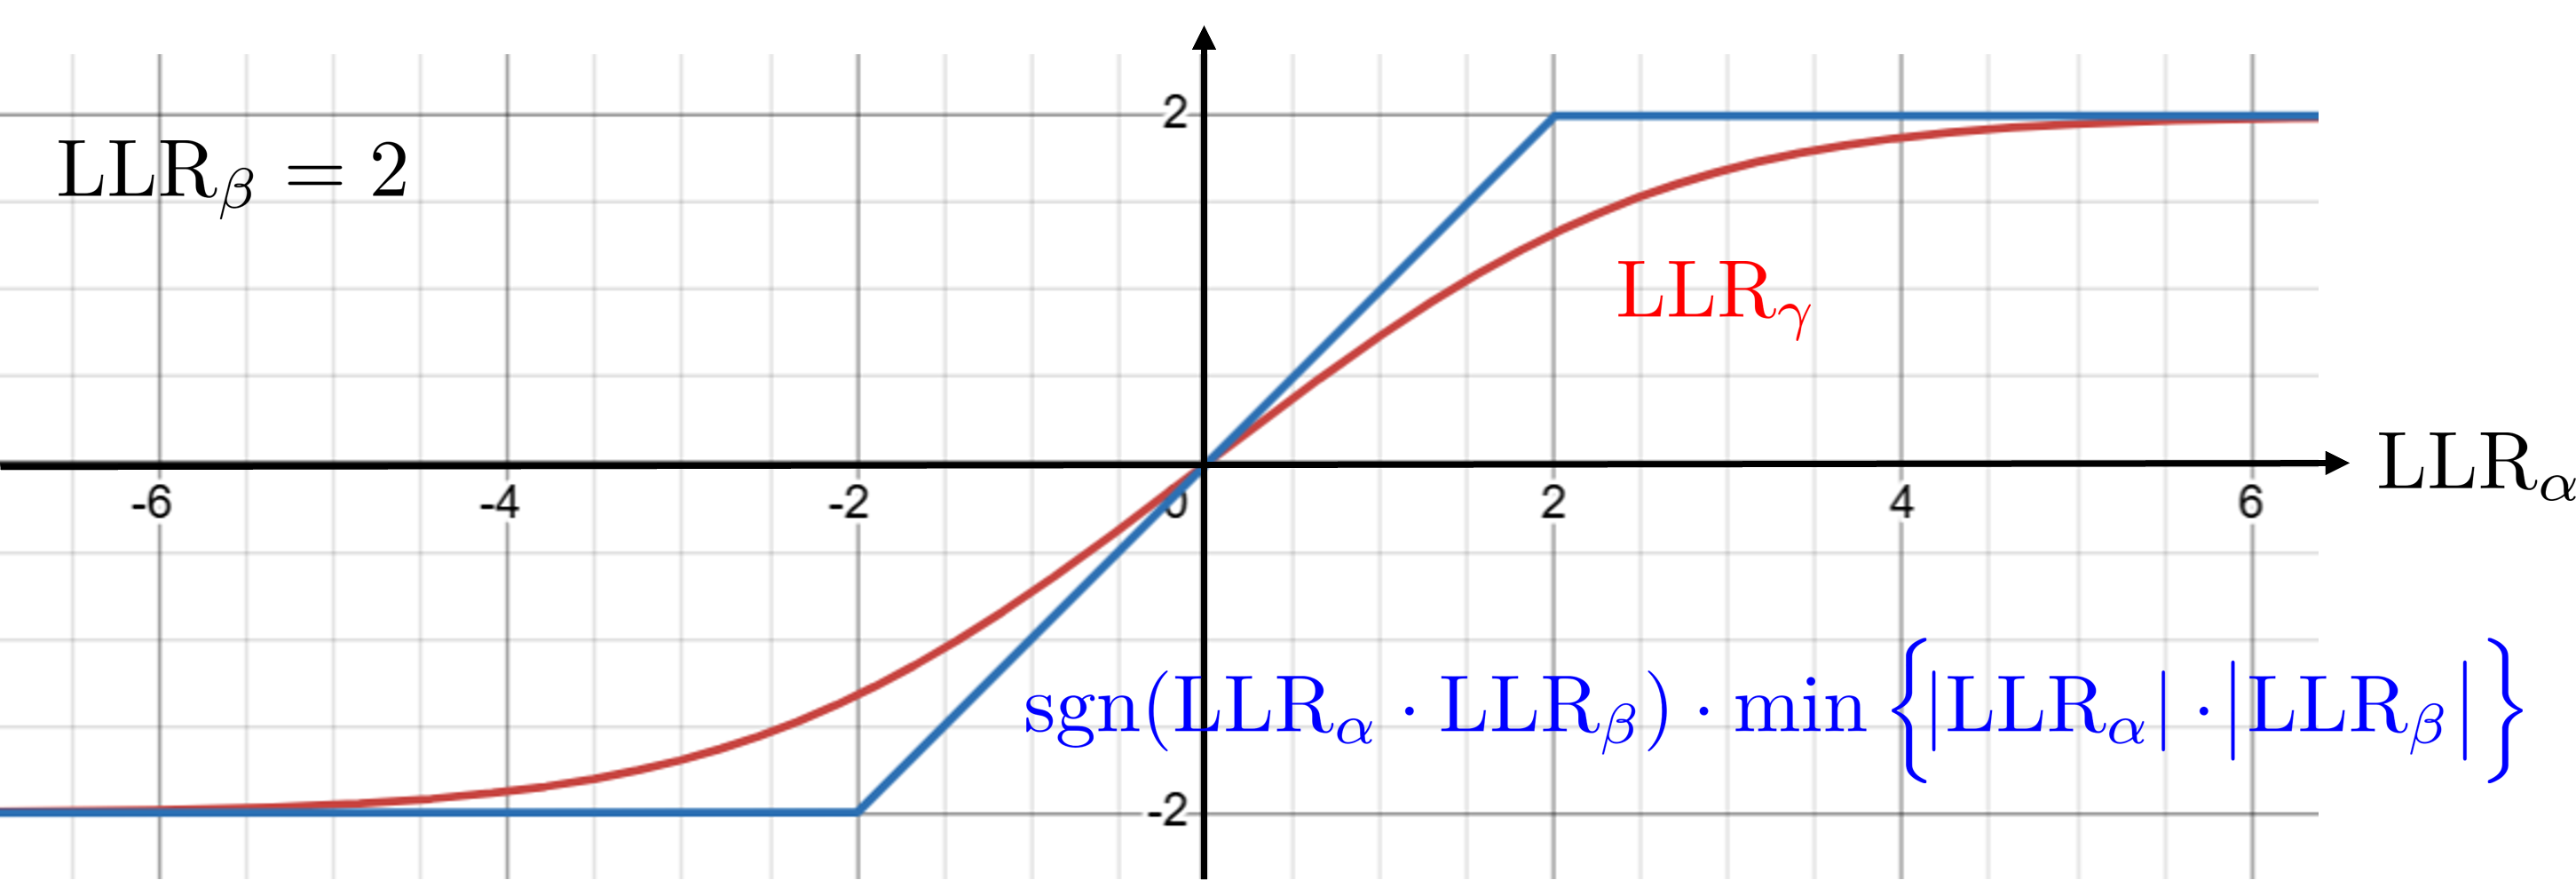
\includegraphics[width=0.7\linewidth]{figures/w5_approx_LLR.png}
    \caption{Approximation for the LLR of serial combination.}
\end{figure}

\begin{example}
    If one flips a biased coin with probability of landing on heads being $p$ a total of $n$ times, what is the probability that the number of heads obtained is even?

    This problem can be solved by using techniques from difference equations. However, we can recast this problem into a channel: Suppose one transmits the bit string $00\ldots 0$ (length $n$) through a $W=\mathrm{BSC}(p)$, then the probability of receiving obtaining an even amount of 1's is the same as the probability in question. This then also equals to the probability that summing (mod 2 summation) the received bits gives you 0. The summation of received bits is equivalent to the serial combination of channels! Since the signed total variation distance (temporarily denoted by $\tilde{T}$) is multiplicative under serial combination, let the probability of obtaining a sum of 0 be denoted by $q$, then
    \begin{equation*}
        \tilde{T}(W^{\boxstar n}) = q - (1-q) = \left((1-p) - p\right)^n = \tilde{T}(W)^n \Rightarrow q = \frac{1}{2}\left((1-2p)^{n} + 1\right).
    \end{equation*}
\end{example}

\section{Distributed Source Coding}
This section discusses the possibility of distributed source coding by the method of Slepian-Wolf.

\begin{figure}[H]
    \centering
    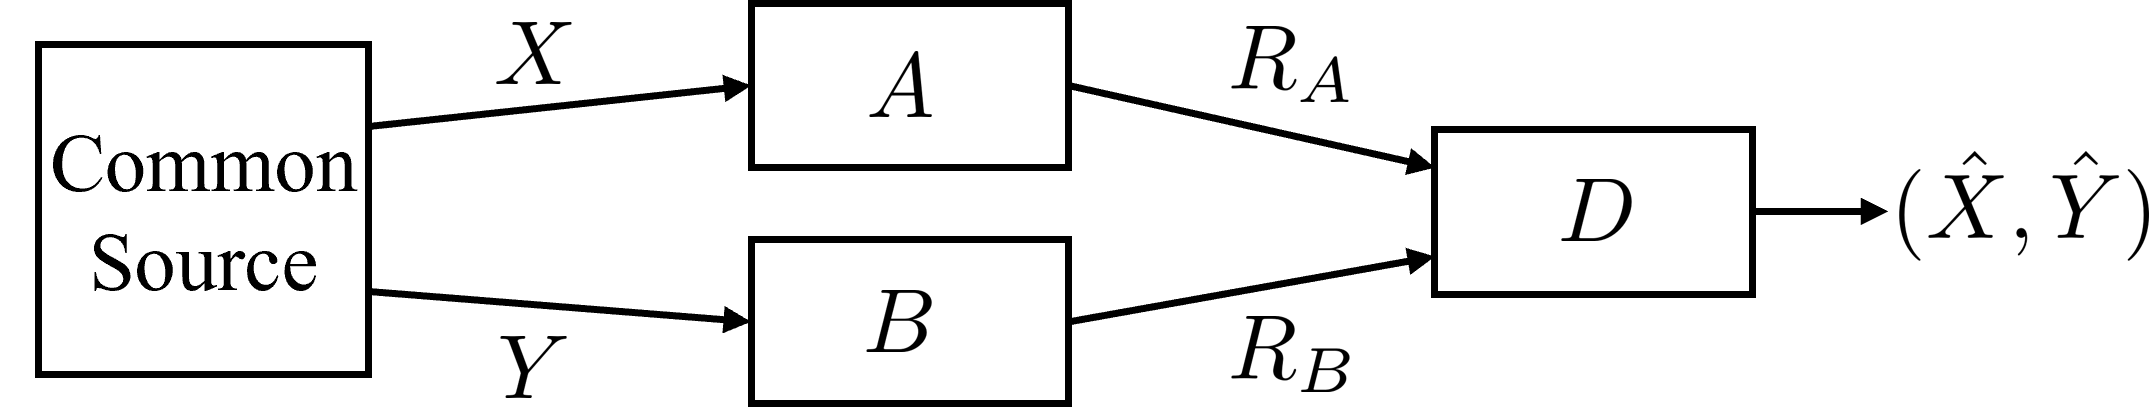
\includegraphics[width=0.6\linewidth]{figures/w5_distr_src_coding.png}
    \caption{Distributed source coding of a common source by two agents $A$ and $B$.}
\end{figure}

Consider the figure above: agent Alice ($A$) and Bob ($B$) has a common source and plan to send bit streams with rate $R_A$ and $R_B$ to decoder David ($D$) to learn about the source. What are the possible $(R_A,R_B)$ pairs?

From \autoref{sec:slepian_wolf_1}, we have learned that if Alice or Bob shares information with the other (say, Alice knows about the random variable $Y$ that Bob obtains), then Alice can send at a rate of $H(X\vert Y)$ while Bob sends at a rate of $H(Y)$. But now our question is restricted so that there are no information exchange between Alice and Bob, is there a way for the them to compress their information while still enabling David to decode the information losslessly? Our task then will be to find a way to describe the \textit{rate region}.

\begin{definition}[Rate Region]
    The rate region is a subset $\mathcal{R}\subset\mathbb{R}^2$ such that $(R_A,R_B)\in\mathcal{R}$ is feasible.
\end{definition}

The characterization to the rate region is the figure below:
\begin{figure}[H]
    \centering
    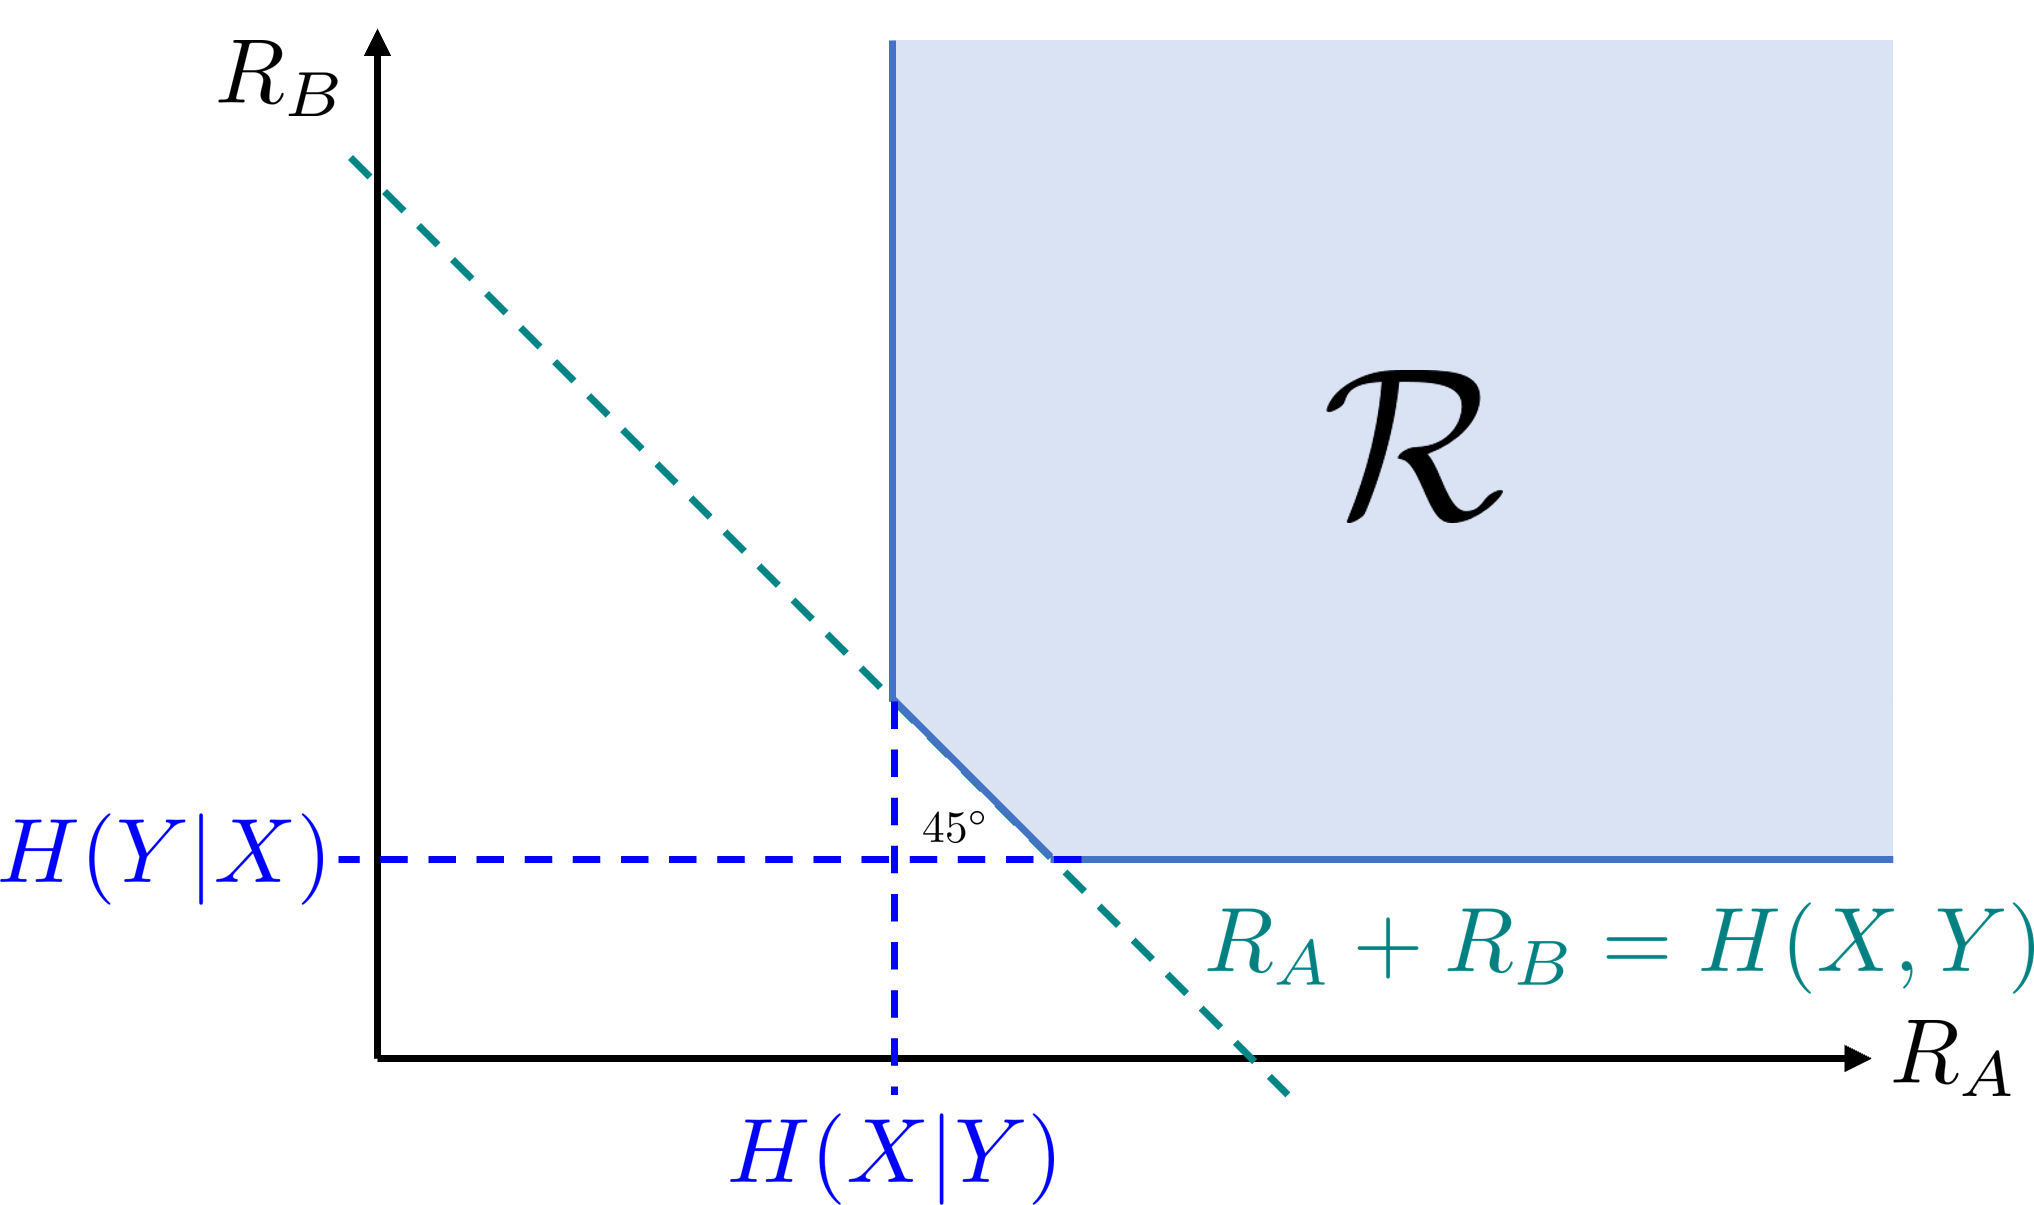
\includegraphics[width=0.6\linewidth]{figures/w5_slepian_wolf.png}
    \caption{Rate region of two agent distributed source coding.}
\end{figure}
\begin{remark}
    The more bits used to describe a single symbol, the more possible it is do decode. Hence, the region $\mathcal{R}$ is unbounded on the top right corner.

    If $X$ and $Y$ are independent, $H(Y\vert X) = H(Y)$ and $H(X\vert Y) = H(X)$, hence $H(X)+H(Y) = H(X,Y)$, the rate region simply becomes an unbounded rectangle.
\end{remark}

The strategy of the coding scheme for Alice and Bob is simple: ask Alice to send bit streams with a rate of $H(X\vert Y)$ and ask Bob to send with a rate of $H(Y)$. An immediate problem arises, however, without explicitly knowing the $Y$ Bob obtains, how can Alice compress the information? Luckily, this task is actually possible, and the technique used is called \textit{random binning}:
\begin{enumerate}
    \item Prepare $2^{n(H(X)+\varepsilon)}$ small balls for Alice. This corresponds to the typical set $\mathcal{A}(n,\varepsilon)$ of information in $X$. 
    \item Prepare $2^{n(H(X\vert Y)+\varepsilon)}$ large bins.
    \item Alice throws the balls into the bins randomly. (Note that if there is no side information, Shannon says that Alice should in fact send David the index of the balls which costs $n(H(X)+\varepsilon)$ bits.)
    \item Alice send the index of the bin a ball is in to David, costing $n(H(X\vert Y) +\varepsilon)$ bits.
    \item In order to show that this trick actually works, David should be able to find the correct ball that is in the bin which has an index Alice sent and David knows.
    \item Each ball is a different random stream of variable $X_{1:n}$. David will select the ball with the largest probability $\mathrm{Pr}\{X_{1:n}\vert Y_{1:n}\}$.
    \item Control and bound the error probabilities:
    \begin{itemize}
        \item The wrong ball has a higher probability.
        \item $\cdots$ (to be left as an exercise for the readers)
    \end{itemize}
\end{enumerate}
By bounding the error probabilities, we can show that the strategy of random binning is feasible, and the error probabilities reaches zero as $n$ becomes asymptotically large.